\documentclass[12pt,letterpaper]{article}

\usepackage[utf8]{inputenc}			% Sets encoding to UTF-8
\usepackage{times}					% Use Times New Roman as the default font
\usepackage{setspace}				% Free document from ugly single spacing
\usepackage{graphicx}				% So image use is possible
\usepackage{enumerate}				% Allows use of specified list numbering (letters)
\usepackage{lastpage}				% Gives the last page number as an accessible number
\usepackage{fancyhdr}				% Makes "1 of 10" type page numbering possible
\usepackage{array}					% Used in the table\usepackage{enumitem}
\usepackage{url}					% Provides clickable URLs (in the bibilography)
\usepackage[sort&compress]{natbib}	% Need this for the bibliography to work properly
\usepackage[margin=1in]{geometry}	% Set margins to standard 1 inch margins
\usepackage{xurl}					% Provides url breaks so urls don't overrun lines
\usepackage[protrusion=true,
            expansion=true,
            final]{microtype}		% Improves hbox handling, reducing errors
\usepackage[breaklinks,
			colorlinks = true,
            linkcolor = blue,
            urlcolor  = blue,
            citecolor = blue,
            anchorcolor = blue]
            {hyperref}				% Makes TOC Links to content
%\usepackage{showframe}				% Uncomment for troubleshooting layout issues

% use the same font for URLs - better than courier...
\urlstyle{same}

% make the text easier to read
\onehalfspacing

% don't want page numbering until the abstract
\pagenumbering{gobble}

% setting up the "1 of 10" type page numbering
\pagestyle{fancy}

% remove the "fancy" header - too cluttered and not in original
\fancyhead{} %remove contents of header
\renewcommand{\headrulewidth}{0pt} % give header no space and thus remove horizontal line

% add the "1 of 10" type page numbering
\fancyfoot[C]{\begin{flushright}\begin{footnotesize}{\thepage} of \pageref{LastPage}\end{footnotesize}\end{flushright}}

% some aliases for organizations in the bibliography who need citations to show up in the references section
\defcitealias{Ocean2021}{Ocean Marketplace}
\defcitealias{Balancer2021}{Balancer Liquidity Bootstrapping Pools}
\defcitealias{EIP-721}{EIP-721}
\defcitealias{EIP-1155}{EIP-1155}

\begin{document}

\begin{titlepage}
\centering
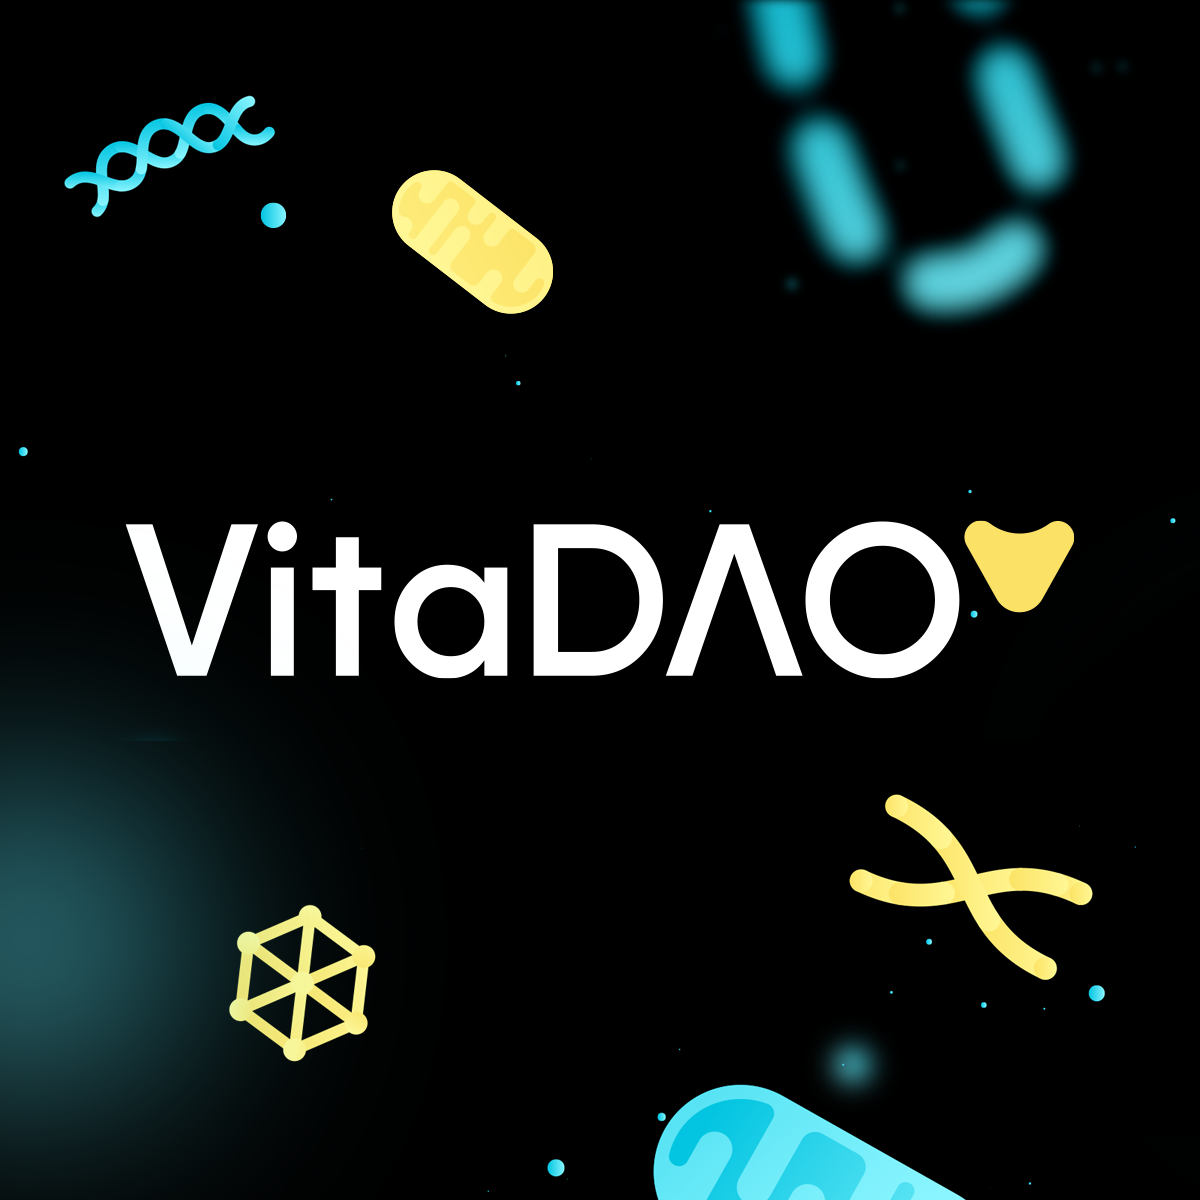
\includegraphics[width=0.8\linewidth]{images/VitaDAO Opengraph.png} 
\\
\vspace{36pt}
{\begin{Large} \textbf{Whitepaper V1.0}\end{Large}}
\\
\vspace{18pt}
{\begin{large}{Authors: Tyler Golato, Paul Kohlhaas}\end{large}}
\\
\vspace{18pt}
{\begin{small}{Editor: Audie Sheridan}\end{small}}
\\
\vspace{18pt}
{\begin{small}{Acknowledgments:  Jesse Hudson, Elad Verbin, James Brodie, Trent McConaghy, Robert Miller, Dimitri De Jonghe, Aubrey De Grey, Morten Scheibye-Knudsen, Theodor Walker, Juri Stricker, Sebastian Brunemeier, Alev Basaran, Tim Peterson}\end{small}}
\\
\vspace{18pt}
{\small\emph{(Draft open for public and community comment)}}
\end{titlepage}

\newpage

%start page numbering on the abstract page
\pagenumbering{arabic}

\begin{abstract}
% make the abstract section number be zero
\addtocounter{section}{0}
% add the abstract to the TOC, preserving section numbering
\addcontentsline{toc}{section}{\protect\numberline{\thesection}Abstract}

VitaDAO is a new cooperative vehicle for community-governed and decentralized drug development and intellectual property. Our core mission is the acceleration of R\&D in the extension of human life and health-span. Today, the biopharma industry booms with unprecedented late-stage investment, particularly in longevity science. However, the industry severely lacks critical early-stage funding. Moreover, incentives between patients, researchers and industry are misaligned, risking a monopolization of lifespan extension.

At its core, biopharma value creation consists of intellectual property (IP) rights, domain specific know-how, and research data. Today, R\&D has become prohibitively expensive and siloed, largely due to the way IP business models incentivize monopolization of innovation. This is done through the creation of patent thickets in protected portfolios. These IP mechanisms prevent open sharing of research data, inherently disincentivizing collaboration and transparency. They prevent the public and patients from having any real ownership in biopharma IP, despite their tax dollars funding most early-stage development. Outside of grants to fund basic research, early-stage funding for drug development is extremely limited. When drugs do finally make it to market, there exist strong incentives for price gouging. 

To align incentives and vitalize early-stage funding in longevity biopharma, VitaDAO uses a combination of novel governance frameworks in decentralized autonomous organizations (DAOs), non fungible tokens (NFTs), and financial engineering tools such as algorithmic automated market makers (AMMs), all of which run on the Ethereum blockchain. 

As an open global cooperative that anyone can join, VitaDAO’s goal is to support and finance new therapeutics and research data in longevity science. In exchange, VitaDAO will directly hold IP and data rights in the novel early-stage therapeutics it supports and funds. We will grow a portfolio of IP and data assets, which we can make available and monetize through novel data marketplaces or by conventional licensing and commercialisation processes in biopharm. By utilising community-guided decision making processes, VitaDAO aims to A) rapidly decrease funding decision lifecycles; B) attract the worlds leading researchers by promoting open science principles; C) democratize ownership thereof.

The lifeblood of VitaDAO is its native curation and governance token: VITA. VITA tokens may be obtained by individuals or organizations by contributing work, funds, or other resources like data and IP. Ownership of VITA allows the holder to participate in the curation and governance of VitaDAOs assets and its research.

\end{abstract}

\newpage
% Make it read "Table of Contents" and center
\renewcommand{\contentsname}{\centering Table of Contents}

% Keep the TOC simple
\tableofcontents

\newpage

\section{Introduction and Key Challenges}
Current biopharma business models carry severe limitations and R\&D inefficiencies at the cost of those who should be the core stakeholders: patients in need of medication and researchers discovering new therapeutics. We propose a novel organisational structure to address these challenges.
 
VitaDAO is a decentralized membership collective funding early stage longevity research. Its mission is to extend human lifespan by researching, financing, and commercializing longevity therapeutics in an open and democratic manner. VitaDAO will own the intellectual property assets that result from the projects it supports, and members of VitaDAO govern the structure and its decision making processes. Members can join VitaDAO by purchasing VITA tokens or earning them through contributions of work or intellectual property.
For a non-technical summary about how VitaDAO works, please see \href{https://vitadao.medium.com/how-vitadao-works-61bbf861fe96}{here}.

\subsection{Longevity Will Transform Our Approach To Medicine}
Longevity science has the power to completely transform global healthcare. Age-related diseases are among the most significant contributors to our global health burden and are responsible for the highest costs incurred by healthcare systems \citep{WHO2011}. 

The longevity space is experiencing a tremendous boom, in part because of its ability to address this problem. The space is evolving rapidly in terms of understanding the aging process and its capacity to develop health and life-extending therapeutics \citep{ARDD2020}. It is now a routine procedure to reverse the aging of human cells in the laboratory. Correspondingly, the economics of investing in longevity are more attractive than ever. There are 100s of new companies and funds dedicated to research and product development in the fields of senolytics, telomeres, stem cells, mitochondria, and gene editing \citep{Pfleger2021}. These are some of the core domains from which therapies that increase lifespan will emerge. However, aging is not recognized as a disease, and this has created barriers to prescribing drugs for aging itself \citep{Suresh2014}). 

The rush of investment into the field has the potential to rapidly accelerate these developments but also comes with distinct problems. The centralization of aging research by large institutions and billionaires has the potential to create the same problems and pitfalls that plague the pharmaceutical industry: lack of transparency, restricted access, and concentrated control over therapeutics that should be made widely available to anyone at an affordable price. 
We believe the future of health and life-extension should be open, collaborative, and community owned. We see longevity as an entirely new approach to medicine, one that has the potential to prevent, as opposed to treat or intervene. This approach will completely change the way the world provides medical care and will profoundly impact society. Moreover, we are at risk of allowing the monopolization of these new technologies, making longevity a luxury good accessible to the 0.1\% globally and preventing redistribution of wealth \citep{Ihle2017}, leading to further income inequality and concentration of capital.

\subsection{Intellectual Property in Biopharma}
Fundamentally, value creation in biopharma consists of two core assets: intellectual property (IP) and research and development (R\&D) data \citep{Chandra2011}. When companies explore a use case for a new therapeutic, they patent their discoveries to gain IP. IP enables them to secure future revenue and recoup the high costs of R\&D. As companies invest billions of dollars into generating data to bring therapeutics to market, they offset this by selling equity ownership or IP royalty rights in the form of future drug sales or milestone based payments. \citep{Wouters2020}. While IP in theory incentivizes innovation, in practice it does the opposite. IP ownership as a business model barely evolved in the past century, remaining mainly extensive legal contracts and bureaucratic complexities. IP is one of the most valuable asset classes in the world but it remains rigid, largely illiquid, and difficult to transfer. 

First, IP owners and sellers who seek to monopolize commercial value have incentives to withhold negative research data. This creates a principal-agent dilemma and, in part, leads to a phenomenon coined the “reproducibility crisis” \citep{Sherkow2017}. Pharma tends to only share positive R\&D data which leads companies to waste enormous resources repeating each others’ failures because without complete data, clinical and preclinical studies are often not reproducible. 

Second, The current system severely lacks incentives for open science, collaboration, and data sharing \citep{Ali-Khan2017}. IP Owners downplay side effects or indicators of lower effectiveness in favor of profit maximization. Valuable research findings are lost for the broader scientific community and not considered during patient treatment. Monopolistic IP ownership within biopharma companies leads to centralization, and the disincentivization of collaboration. Promising drug candidates often fall to the wayside for organizational, political, or competitive reasons. These centralized and siloed research efforts lead to the high R\&D cost and long time-to-market plaguing pharma today. The excess cost ranges from \$800 million to \$2.6 billion on average in cost, and time to market takes upwards of 10 years  \citep{DiMasi2016}. On a macro scale, this IP model leads to incentive misalignment and information asymmetry. 

Lastly, the current financing and investment landscape restricts access and participation to early-stage biopharma from its most important stakeholders: patients and researchers. In the US, generally only accredited investors can finance early-stage ventures \citep{Rowley2018}. The market is opaque, and no singular or efficient marketplace exists to discover or access these opportunities in a transparent fashion.

We need more democratic, open, and transparent models. Collaboration and open research in the scientific community could bring down the rising cost of drug development \citep{Bookbinder2020}. 

\subsection{The Evolution of Pharma and the Valley of Death}
There is a significant shift underway in the pharmaceutical industry’s process of drug development. Increasingly, smaller biotech firms leverage recent academic research in the life sciences to develop new drugs, and then pharmaceutical giants acquire these smaller firms and their expertise using their access to low-cost capital \citep{Huang2021} Notably, much of the funding for this academic work comes from grants or public capital, but pharmaceutical companies then privatize it so the public receives little upside from the research it funded \citep{Toole2004}. The number of biotech startup companies formed due to technology licensing increased dramatically in recent years, from 145 in 1994 to 278 in 2000 to 1,024 in 2016. The increase is on an exponential curve. Of the 30 top-selling drugs worldwide in 2000, only five traced back to universities and the remaining 25 were developed by big pharma. By 2018 however, more than half of the top 30 drugs were sourced from academia \citep{Huang2021}. Biotech universities increasingly prove themselves as untapped goldmines of valuable IP, yet often these assets are unavailable for investment until a startup spins up. 

Assets from universities not out-licensed or spun out into startups remain in a difficult limbo, known as ”The Valley of Death,” where they often fail to move forward \citep{Seyhan2019}. Many of these technologies have extreme value to patients, but because of this system, they never ultimately serve the populations intended to benefit from them. These assets require investment and capital injections at a much earlier stage. The market desperately needs new open commercialization models to incentivize their development. 

\section{Solution}
To address some of the core problems mentioned above, we propose the creation of VitaDAO: a new cooperative vehicle for community-governed and decentralized longevity drug development. VitaDAO is a decentralized organisation incorporated via smart contracts on a distributed ledger and virtual machine. DAO frameworks follow years of research and experimentation in decentralised governance systems, open networks and decentralized financing solutions. The methods proposed below, while radical, have been adequately tested in other scenarios and are ripe for tackling this core issue.

Anyone can govern VitaDAO by acquiring VITA governance tokens through the contribution of funds or by earning it through the contribution of work, research data, IP assets, or services to VitaDAO. VitaDAO will acquire IP rights and R\&D data, and also commission research to further develop its assets. VitaDAO’s core assets will consist of: 

\begin{enumerate}
\item IP; including patents and licenses to therapeutics. 
\item R\&D data assets generated by funding research projects. 
\item Funds stored in its treasury, including unissued VITA.
\end{enumerate}

VITA is designed as a governance and curation token. Ownership of VITA allows the holder to participate in the governance of VitaDAO, and thus, direct its research, access and monetize its data repositories, and manage its IP portfolio.

To acquire and finance specific research proposals, VitaDAO members may elect to issue tokens. VitaDAO can do this on a continuous or per-project basis, using automatic market makers (AMMs) like \citetalias{Balancer2021} (LBPs) that enable a fair and transparent participation for prospective members. 

In order to curate, govern and monetize IP and data assets on a decentralised network, VitaDAO utilises Non-Fungible Token legal frameworks (NFTs) such as \citetalias{EIP-721} and \citetalias{EIP-1155}, as detailed below in Section 4.

\subsection{Stakeholders}
VitaDAO will rely on collaboration between members, working groups, and service providers to facilitate all functions of the DAO.  

\subsubsection{Members}
A member of VitaDAO is any entity that stakes VITA into VitaDAOs governance smart contract to participate in voting. Initially, tokens can only be obtained by providing funds or work to the structure. Members have full governance rights and can participate in governance on Discourse (informally) and via token-based voting (formally).

\subsubsection{Working Group Members}
A working group member provides expertise and advice to VitaDAO. Members can apply to join working groups based on their experience or expertise. Working groups elect working group stewards, which are responsible for leading working groups. Working groups can opt to create incentives for their members, or pay them for services and/or create bounties. In cases where working group members are paid, group members can be compensated in VITA, cash, or other incentive schemes decided by members.

\subsubsection{Working Groups}
\begin{enumerate}
\item Governance
\item Tokenomics
\item Information \& Awareness
\item Legal
\item Longevity
\item Compensation/Incentives/Ops
\end{enumerate}

\subsubsection{Service Providers}
Members who provide services to VitaDAO, such as development work, IP sourcing, and conversion to NFTs, marketplace services, drug development services outside of project scope, etc. Service providers are typically paid for their services in fiat or offered tokens in exchange.

\vspace{15pt}
\begin{center}
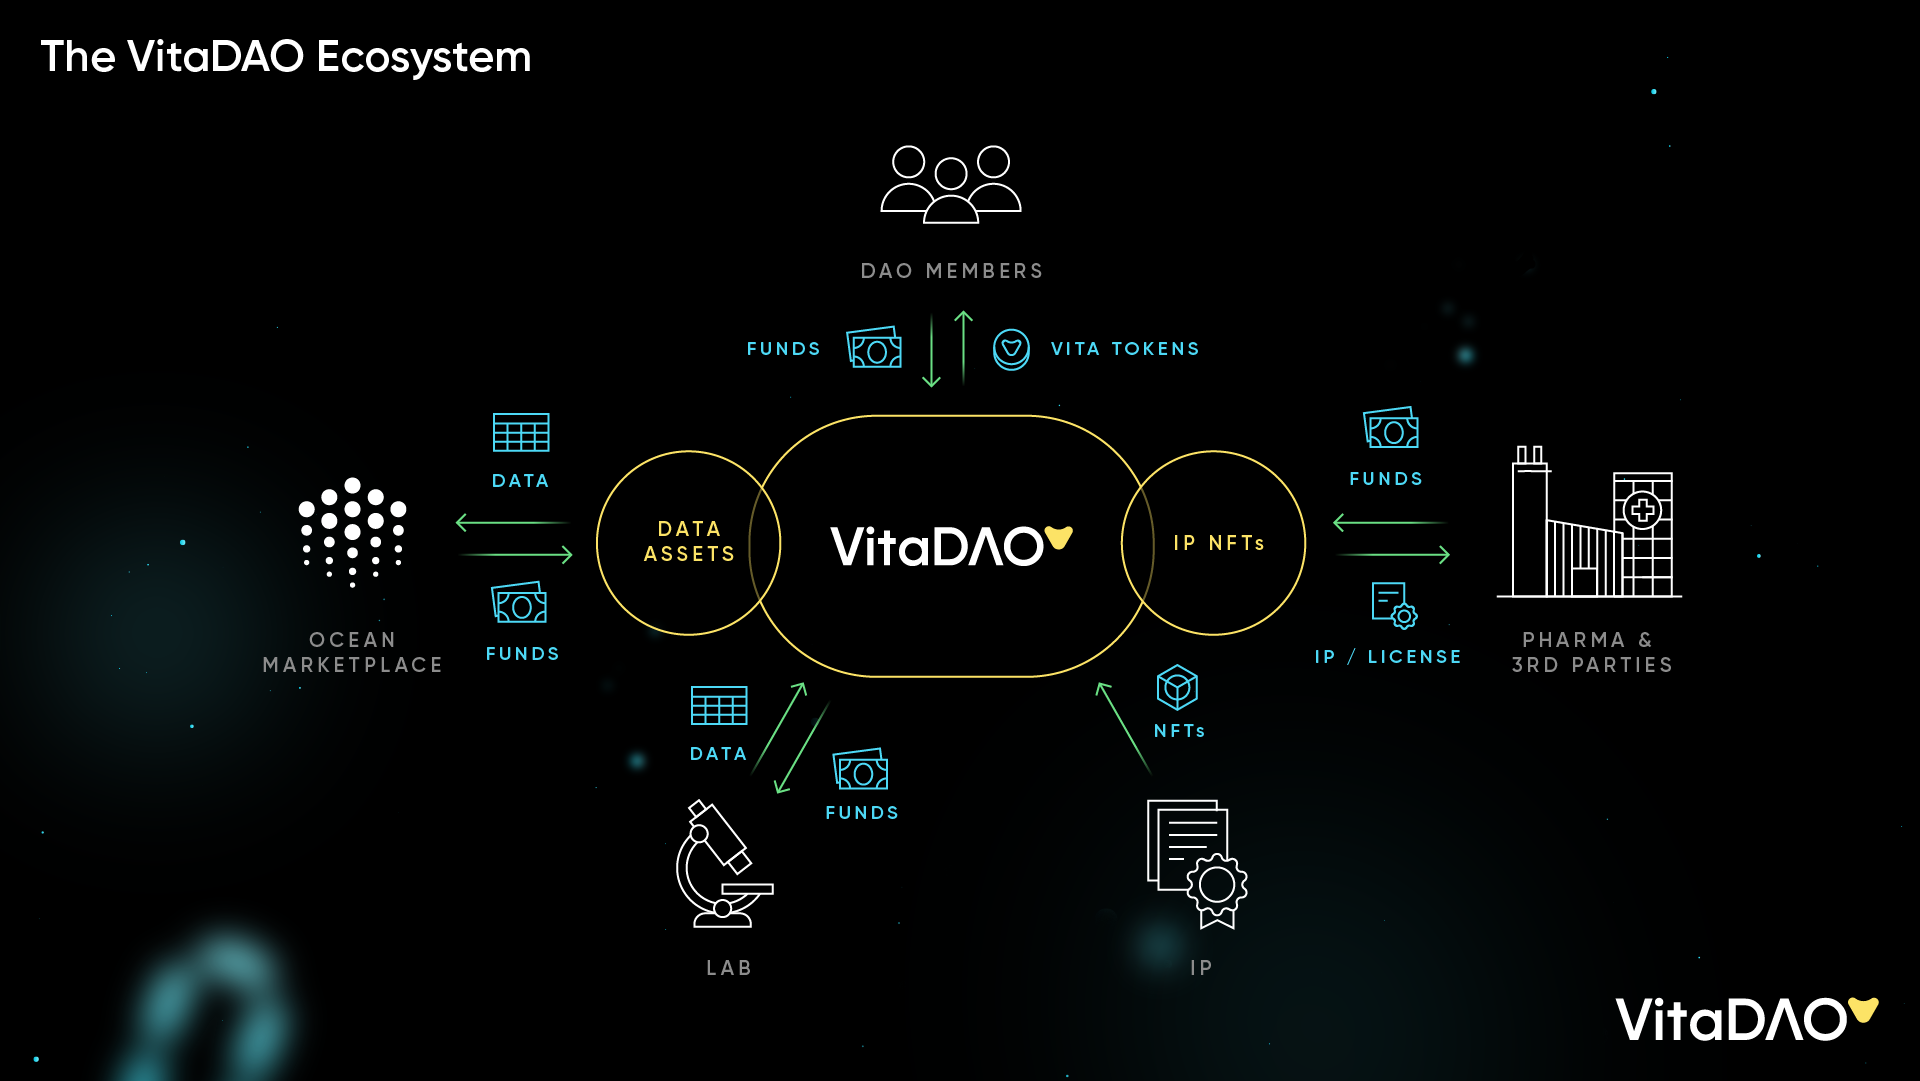
\includegraphics[width=\linewidth]{images/VitaDAO Diagram - Ecosystem-p-1600.png} 
\end{center}

\section{Core Architecture}

\subsection{Architectural Summary}
VitaDAO operates via smart contract on the Ethereum blockchain. VitaDAO V1 consists of several core components including: 

\begin{enumerate}
\item VitaDAO’s governance smart contracts, modeled after MolochDAO and the LAO.
\item VitaDAO’s contribution and bootstrapping mechanism utilizing Gnosis Auction. 
\item VitaDAO’s native governance token, VITA.
\item VitaDAO’s IP and data assets, which are represented as NFTs. 
\end{enumerate}

VitaDAO’s smart contract architecture enables members who own VITA to freely engage in governance decisions pertaining to the assets and funds held by VitaDAO. Members will manage VitaDAO using a decentralised application, through which they will interact with VitaDAO’s smart contracts and facilitate the purchase, funding, and management of IP and data assets.

\subsection{Governance Framework Overview}
VitaDAO members are in control of all governance decisions by voting on VitaDAO proposals. Proposals can be made by any VitaDAO member. VitaDAO members can create proposals by posting in the “proposals” section on Discourse, gaining community support, and eventually electing to put the proposal to a token-based vote. 

VitaDAO working groups consist of domain experts to help guide member decisions in various work streams and organisational processes. Working groups can help define proposals to the VitaDAO members. VitaDAO may engage service providers spanning patent attorneys, contract research firms, or third party experts to provide services to the DAO in exchange for compensation.

The initial goal is to mimic successful execution patterns in the biotech industry. Over time, we expect further governance mechanisms to emerge around VitaDAO.

\subsubsection{Proposal Process Summary}
Proposals are the primary means through which the DAO makes decisions, deploys funds, and adapts behaviors. Proposals can be made informally or formally by various means. Discord is the primary place where informal discussions are held. If these discussions lead to the need for a proposal, a first draft of the proposal should be uploaded to Discourse for community input. These soft proposals are later refined based on community input and reuploaded to Discourse as a final draft. If needed, the proposal can be uploaded to the VitaDAO application for a formal, token-based vote. 

To accelerate decision making, made using a soft governance mechanism via Discourse, particularly such decisions that can be adapted by norm-setting and don’t require the DAO to issue funds or tokens from its treasury. However, in core cases, such as when a funding decision needs to be made, a token-based vote is required. The process for creating proposals is as follows:

\begin{enumerate}
\item Phase I (Draft): Post V1 proposal to VitaDAO Proposal Channel in Discourse for community feedback and input.
\item Phase II (Refine): Post refined and polished V2 proposal to VitaDAO Proposal Channel in Discourse based on feedback and community input received.
\item Phase III (Final): Upload to platform for token-based vote if necessary.
\end{enumerate}

\noindent For more detailed information and user flows, please visit \url{gov.vitadao.com}.

\subsection{VITA Token Economy}
The VITA token is the lifeblood and DNA of the VitaDAO ecosystem. VITA is obtained by contributing work, data, IP, or funds to VitaDAO. The core function of VITA is to curate the best longevity IP and fund novel open science data creation around it.

VITA tokens grant the rights to participate in: 1) which IP is funded; 2) how it is funded; 3) how it is governed; 4) how the VitaDAO treasury is governed. As such, VITA grants no ownership of the IP but full governance rights. It is the active duty of VITA holders to decide how all of its R\&D projects may be commercialised and brought to patients.

VITA is designed following a sustainability loop principle \citep{Web3Sustain}. As R\&D projects are funded and begin producing data, the IP value may grow if positive research results. If the VITA ecosystem grows, more funds become available, attracting higher quality IP and enabling the funding of further projects and growing the VitaDAO ecosystem.

\subsubsection{Genesis}
The diagram and table below propose the initial VitaDAO token distribution. Overall, 30\% will be distributed to the community for the initial genesis, whereas 70\% of tokens remain available unminted in the VitaDAO treasury to ensure the longevity of the entity. The initial genesis auction should be considered the first proof of concept financing to prove VitaDAOs IP and funding model. Members may elect to issue further tokens at any time to the public or select strategic entities and funders. Furthermore, tokens may be allocated to various incentive schemes and mechanisms as proposed herein.

\vspace{15pt}
\begin{center}
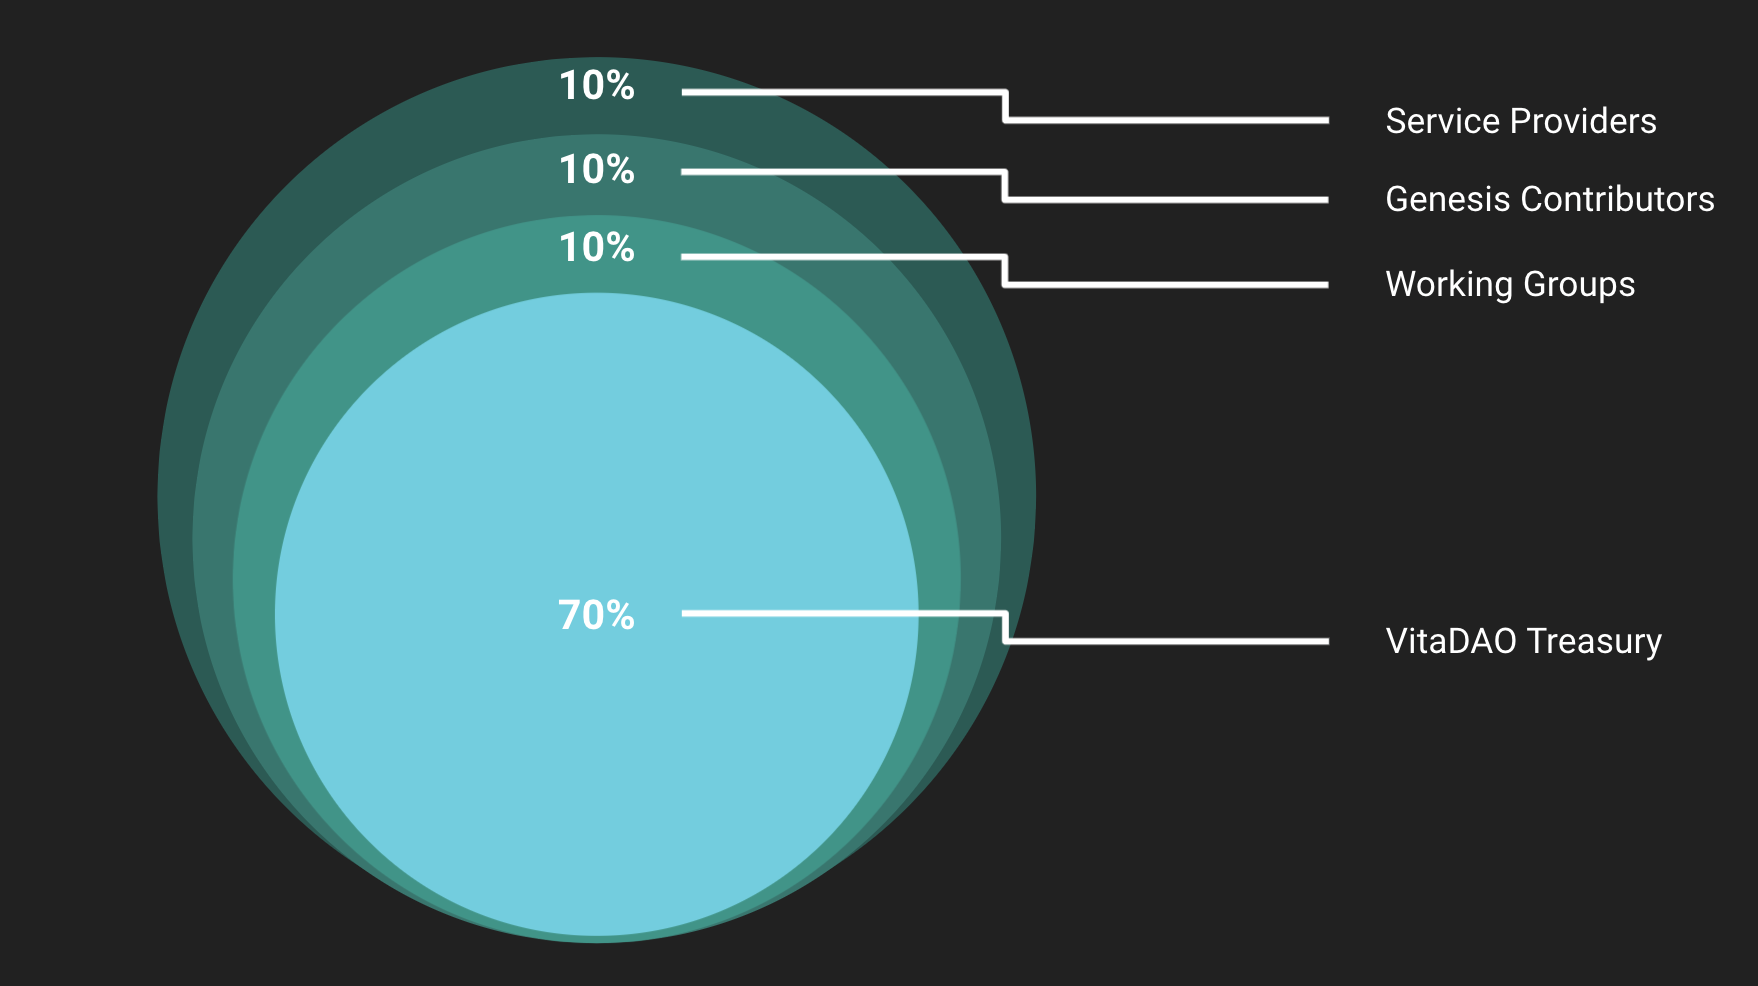
\includegraphics[width=\linewidth]{images/Initial Token Allocation.png} 
\end{center}

\subsubsection{Token Supply and Distribution}
Jeanne Louise Calment is the oldest person to have lived for a period of 122 years and 164 days. She lived approximately 64,359,360 minutes on planet earth, which will form the basis of VitaDAO’s DNA. Upon genesis, 64,359,360 VITA will come into existence as a native ERC20 token controlled by VitaDAO. VitaDAO’s token supply is capped. We propose this may only ever be considered to increase, should anyone extend her lifespan - forming our core collective mission at VitaDAO.

\begin{table}[h!]
  \begin{center}
    \setlength{\extrarowheight}{5pt}
	\begin{tabular}{p{0.2\textwidth}p{0.2\textwidth}p{0.3\textwidth}}
		\textbf{Tokens} & & \textbf{Stakeholder}s \\ 
		\hline
		6,435,936 & 10\% & Community Genesis \\ 
		6,435,936 & 10\% & Service Providers (Voted) \\ 
		6,435,936 & 10\% & Working Groups (Voted) \\ 
		45,051,552 & 70\% & Treasury \\ 
		\hline 
		\textbf{64,359,360} & \textbf{100\%} & \textbf{VitaDAO} \\ 
		\hline 
	\end{tabular} 
  \end{center}
\end{table}

The genesis distribution event will liberate 10\% of VitaDAOs total token supply to interested participants fully open to the public via interaction with a smart contract auction system on the Ethereum blockchain.

Since VitaDAO operates via a public auction system, the token price is dictated by the community. We estimate that a minimum of \$2,500,000 will be required to support the first cohort of research projects and form the base requirement of a successful auction.

VitaDAO will be fully decentralized and community-owned from inception. As such, no entity will own VITA tokens prior to the genesis contribution event. No tokens have been issued or sold to individual contributors, as nobody controls VitaDAO until inception.

VITA’s genesis contribution event will run via a fair launch public auction, granting all participants equal governance rights. Once the first 10 \% have been issued, the VitaDAO core community may begin voting on its first governance proposals to allocate further tokens to working groups and service providers.

Importantly, the approval of these allocations to working groups, contributors, and service providers is at the full discretion of genesis members and their approval. They form the core of VitaDAOs decision-making and executive body.

\subsection{Community Genesis Auction}
VitaDAO intends to launch in a fully fair and transparent manner, favouring community participation over centralised entities. As no one is in control of VitaDAO, no tokens have been issued or promised to external entities.

As a first step, VitaDAO will enable any interested member of the public to contribute to its genesis period utilising a Gnosis Auction mechanism.

Gnosis Auction uses batch auctions \citep{BatchAuctions}, which are an economic design mechanism for ensuring fair price discovery. Batch auctions enable matching of limit orders of buyers and sellers with the same clearing price for all participants. From web3 use cases like Initial DEX Offerings (like those on the Mesa interface for Gnosis Protocol v1) to traditional commercial and financial auctions (like Google’s IPO and the NYSE Open Auction), batch auctions play an important role in the democratization of the auctioned assets. This function is especially important for decentralized entities which need to ensure fair token distributions while operating trustlessly and efficiently. Batch auctions are set to become a fundamental building block for collectives and communities interested in offering their users a transparent and fair auction and price-discovery mechanism. In practice auctioneers determine a minimum price they are willing to sell a fixed amount of tokens for. Bidders set the maximum price they are willing to pay for a fixed contributions. These characteristics allow the platform to create a fair pricing dynamic in which both participants get either what they were willing to receive or more.

VitaDAO’s initial genesis will operate as follows:
 
\begin{enumerate}
\item VitaDAO will allocate 10\% of its fixed token supply into a Gnosis Auction with the goal to raise sufficient funds to finance a minimum of five projects and enable the DAO to cover operational expenses and running costs. The community will decide on the full fundraising budget and structure pending simulations and crypto economic modeling using cadCAD. 
\item The Gnosis Auction allows the community to contribute funds and join VitaDAO for the first time. Gnosis Auction is a platform enabling fair price discovery for token auctions. The aim of the platform is to make it easy for VitaDAO to discover a fair price for its token. 
\item After a fixed period, the Gnosis Auction ressolves, forwarding its acquired funds to VitaDAO and kick starting its operation. Should the Gnosis auction fail to reach a specific threshold, participants may withdraw their stakes.
\end{enumerate}

VitaDAO’s genesis auction will be modelled on a minimal funding assumption, but otherwise follow full transparent launch mechanisms. Once the auction completes, VitaDAO members may decide to initiate various other fundraising mechanisms such as Balancer Liquidity Bootstrapping Pools or OTC issuance of VITA to selected parties at the full discretion of its community. The VITA token will be in complete control of its community upon genesis.

\section{Staking and Signaling}
Members can use VITA tokens to signal long-term support for individual projects. A member may stake their VITA tokens for a set time period until a project milestone is reached (e.g. 3 months/6 months/12 months). Projects predetermine milestones and they must be measurable. Their outcome is uncertain, however, meaning members take additional risk by foregoing liquidity. 

When a project reaches a milestone, staked tokens unlock. In return for locking tokens, VitaDAO pays out regular signaling rewards to stakers. This process sends valuable signals to the market, as it showcases the confidence of members in specific projects. Furthermore, it reduces volatility and creates a circular economy to members, who actively contribute value and review project success. 

We anticipate implementing signaling after the first successful project runs an initial funding cycle, giving members time to sufficiently model this mechanism and implement it in VitaDAO V2.

\section{Holding and Managing IP and Data Assets as NFTs}

\subsection{Intellectual Property Rights}
VitaDAO will directly hold IP rights in underlying research projects and will develop a growing portfolio of assets represented as NFTs using a novel biopharma IP NFT framework developed by Molecule \citep{Kohlhaas}. Molecule’s IP NFT legal mapping framework allows the holder of an existing piece of IP, in the form of a license or patent, to be attached to an NFT and transferred to a new owner within seconds. Digital asset identifiers to IP are stored on immutable file storage networks, such as IPFS \citep{IPFS} and Arweave \citep{Arweave}. Furthermore, sensitive data can be protected and obfuscated to only be accessed by the holder of the NFT, as would be the case with a legal license. Data can be made accessible via access right management frameworks on local federated data storage systems.

Upon IP NFT creation, the creator must sign a cryptographic message that prints their signature onto an IP licensing agreement. When the NFT changes owners, the transaction requires both buyer and seller of the NFT to sign a message that references the IP license agreement, which includes references to the transaction, the buyer and seller’s respective identities, and legal signatures modeled after the legal Signature Algorithm pioneered by \citep{OpenLaw2019}. 

Initially, VitaDAO will hold IP in research projects for longevity therapeutics in the form of licenses. These licenses enable VitaDAO or its designated service providers to file for patents, monetize the IP, and contract researchers to grow the value of the underlying assets. 

\subsection{Data Assets}
Besides owning IP rights related to individual projects, VitaDAO will also own data assets and research outputs from the R\&D it funds. VitaDAO will hold custody over these assets, while making them available to its members and others, and monetizing them via data marketplaces such as Ocean Marketplace. VitaDAO may attach these data assets to NFTs where useful and applicable.
 
VitaDAO’s introduction of its data assets into Web3 will drive fluid price discovery and liquidity for each individual data set as buyers and sellers engage with them and curate the most valuable findings. Obfuscation of data assets and enabling secure computation on them will be a highly relevant future use case that Web3 protocols such as Ocean Protocol could facilitate. The applications around composability and interoperability here are manifold, and once VitaDAO is live those applications will receive further exploration. 

Data assets could include, but are not limited to: laboratory updates and reports, processed data, quarterly updates, western blot data, qPCR data, cell culture experiments, survival analysis, sequence data, western blot gels, microscopy and cell culture. These data assets could be in the forms of raw data, images or PDFs. 

The type of data assets and their monetization potential are summarized below:

\begin{enumerate}
\item \textbf{Public Data Assets:} All data in these assets are view-able by members, who can vote to list these data packages on various data marketplaces.
% NEXT ITEM NEEDS SOURCE
\item \textbf{IP Data Assets:} Required for filing of patents or further IP. These assets will be obfuscated as they could compromise filing of IP. These assets could end up on data marketplaces after they have IP filed to protect them.
\item \textbf{Progress Data Assets:} Intended to keep DAO members up-to-date on ongoing research findings and serving as proof of progress. This data has a certain level of obfuscation, meaning any information capable of compromising the intellectual property itself will be hidden. Such data would not be relevant for data marketplaces.
\end{enumerate}

Members wishing to engage with the IP, review the data assets directly, or engage with the longevity working group may need to submit KYC documentation and sign non-compete and confidentiality agreements to help ensure the viability of the assets for all members.

\section{Genesis \& First Project Lifecycle}
Within the genesis service provision, we propose to fund VitaDAO’s first end-to-end proof of concept with the Scheibye-Knudsen Laboratory at the Aging Research Lab at the University of Copenhagen.

In a first proof of concept, Molecule has out-licensed the full rights to this project and will transfer it to VitaDAO. In addition, VitaDAO will fund the first set of laboratory experiments and begin receiving its first data assets. We propose to conclude this as a once-off deal to kickstart the VitaDAO research economy. Both the IP NFT transfer and contract research agreement will be submitted to VitaDAO members as an initial vote.

The project lifecycle could operate as follows:

\begin{enumerate}
\item VitaDAO proposes to purchase the Scheibye-Knudsen Laboratory IP NFT.
\item VitaDAO members vote on the proposal and define the project parameters and payment schedules with the Scheibye-Knudsen Laboratory.
\item The project commences as VitaDAO completes a first payment to initiate the preclinical studies.
\item The Scheibye-Knudsen Laboratory begins delivering first data assets consisting of progress reports, raw data and initial findings.
\item First definitive findings are in, and VitaDAO members, supported by working groups, decide how to use the data and further commercialize the asset. This could result in: 
\begin{enumerate}[a.]
\item Filing for further IP and patents.
\item Filing for clinical trials and further studies.
\item Monetizing the data sets through Ocean Marketplace.
\end{enumerate}
\end{enumerate}

VitaDAO will open applications for additional research projects upon launch based on criteria that are currently being refined by the various working groups. To review the current proposals from the longevity working groups and to better understand the evaluation criteria, please visit \url{gov.vitadao.com}.

\section{Exit Scenarios and IP Commercialization}
If the research data surrounding an asset is sufficiently positive and clinical trials are attractive, VitaDAO can license or sell its IP or data to industry stakeholders, such as pharmaceutical or biotech companies. Given enough liquidity and governance sophistication, VitaDAO could even attempt to bring these assets to market itself. Members of VitaDAO will decide on how to distribute income generated from successful IP monetization. 

Individual IP and NFTs may be spun out into separate fractionalized markets to enable more granular participation by the public. From a technical perspective, this would entail moving the NFT and associated data sets out of custodianship of VitaDAO and into a sub-DAO represented by a new ERC20 token. Members of VitaDAO may elect to spin out a project to:

\begin{enumerate}
\item Enable the project and IP to raise additional funding from a wider community.
\item Create exit scenarios for VitaDAO and further decentralize project ownership.
\item Enable more granular fundability and participation on a project level.
\end{enumerate}

\subsection{Pathways to Filing for IP}
The VitaDAO community and working groups should actively collaborate with projects they support to establish an intellectual property protection plan before commercializing. Pathways towards filing IP should be identified early on, if possible. The legal and longevity working groups should guide the community and active projects to help make intellectual property protection decisions and create a clear commercial pathway for the project.

VitaDAO may license it’s technologies to a third-party company to further develop and commercialize it. This can be carried out at any stage if there is interest from a third party. In the long run, the DAO should build internal TTO-like capacities, in the form of collaborative working groups and service providers, to carry out this function. Such license agreements will assign responsibility for paying for patent coverage to protect the invention, set a fee or royalty schedule, and clarify ownership of further improvements or developments.

There are several pathways to IP protection, each with their own advantages and disadvantages. Projects that have the potential to yield composition of matter patents, or New Chemical Entities, are often more valuable than method of use patents. However, new method of use patents will be more common in the context of repurposing projects, which also have distinct advantages, given these drugs have already been tested and approved in humans. This reduces hurdles in the clinic, but may be more difficult to commercialise. Medicinal chemistry strategies can also be employed to create NCEs from repurposed drugs. 

%CONSIDER SUMMARIZING THIS SECTION
To secure a composition of matter patent on a chemical structure, it is necessary to check whether this compound has been previously synthesized and described in the literature. The patent databases (Patentscope, Google Patents) should be consulted to determine whether a compound is truly a new structure and previously undescribed. The SureChEMBL tool should be used to search the chemical Markush structure and substructures of published patent applications. Findings should be made in consultation with an experienced biotech and pharma focused patent attorney at a leading IP law firm. Questions about ‘patentability,’ ‘novelty,’ ‘unity of invention’ and other legal frameworks should be evaluated by this attorney.

\subsection{Pathways to Commercialising IP}
Projects submitted to VitaDAO should specify potential pathways to IP protection and commercialization at the point of submitting an application. This should be high level and subject to change, but will encourage academics to think in the context of a commercial framework. The legal and longevity working groups should evaluate the feasibility of these plans, and provide feedback and guidance on the projects to determine if such a route is feasible. If the route is not deemed to be feasible, the working groups should engage in conversation and provide alternative suggestions. 

NCEs should be prioritized above pathways focused on claiming a new method of use. If a pathway for a new method of use is determined to be a good fit, legal counsel should begin exploring possibilities for optimization early on in the life cycle of the project. 

When a project has sufficient data and support to file a claim on IP, the DAO’s legal counsel should be engaged to determine the best route forward, and to make decisions on which jurisdictions to file in first. The DAO can elect representatives to file these claims on its behalf, or establish legal entities to do so (such as a Delaware LLC). These representatives or entities could also serve as a point of engagement or contracting if these technologies are to be acquired or licensed in the future. Once IP has been filed and a patent is pending/granted, the DAO can engage in BD to license or sell this intellectual property.

The objective of any deal should be to create a “win-win” deal for VitaDAO and potential licensees (pharmas, biotechs, and VCs).

To achieve it, business development executives (WG members, in the case of VitaDAO) on both sides of a licensing deal must ensure that they strive for a fair deal structure, which means that both sides of the licensing deal have to make sure that:

\begin{enumerate}
\item VitaDAO receives payments reflecting the invested money as well as the current product value.
\item The licensee is compensated for taking the risk associated with the future product development.
\item The selected valuation model is transparent and the rationale behind the used assumptions is clear and based on solid data.
\end{enumerate}

Even though it is paramount to get each step in the deal-making process right, one is particularly important: the product value. Without a realistic product value, there is a high risk that the value gap between the licensor and the licensee will be too large to reach a consensus. Product value should be determined by engaging external service providers and experts to the DAO, along with the appropriate WGs. The risk-adjusted Net Present Value (rNPV) valuation method is highly suitable and widely accepted for calculating the product value. The model is clear, transparent and allows one to consider different deal structures, while understanding how the value is split between the licensor and the licensee.

\subsection{Potential Steps for Successful Licensing and Business Development}
\begin{enumerate}
\item Lead generation
\item Shortlisting of companies based on synergy and interest
\item Connecting with the key personnel at the target company (Head of BD \& Licensing, CSO, CEO, Sourcing/Procurement Head, BU/Country Head etc.)
\item Receiving/sharing the IM (Information Memorandum) /NCIP (Non-confidential Information Package)
\item Signing confidential disclosure agreement (CDA) / non-disclosure agreement (NDA)
\item Receiving/sharing CIP (Confidential Information Package)/CIM (Confidential Information Memorandum)
\item Non-binding offer from either party – term sheet
\item Due diligence through data room/face-to-face meeting/ onsite visit/virtual server/black book
\item Negotiation of financial terms; finalize business case; Internal approval of NPV, ROI etc.
\item Signing definitive agreement / MSA (Master service agreement)
\end{enumerate}

\section{Open Research Questions}
The mechanics described in this paper are novel, experimental, and rely on multiple moving parts, especially the creation of an active tokenized governance community. Our goal is to tackle these questions together as a community and through multiple working groups that include industry experts, as these experts will substantially improve the system’s long-term potential.

\begin{enumerate}
\item \textbf{Governance and effective collective decision-making on drug development projects:} can a decentralized community effectively govern and attract the expertise required to successfully commercialize therapeutics? Will the token-based voting mechanism described herein succeed in generating positive outcomes?  
\item \textbf{Biopharma business logic:} will the biopharma industry be open to purchasing IP and patents produced by a decentralized collective, as opposed to current business practices? Will VitaDAO be able to support a sufficient number of projects to become positive-sum at scale?
\item \textbf{Legal and patent law:} can VitaDAO successfully file for further patents on the IP assets it manages or will it have to rely on third parties? In case of patent litigation against VitaDAO, is it able to protect the validity of the IP as a normal company could?
\end{enumerate}

\section{Conclusion}
The open IP and data ownership structures presented here could help alleviate some of the most severe challenges in the current pharmaceutical and biotech pipeline, and could help create a future of open and democratic ownership of longevity therapeutics. 

IP collectives like VitaDAO can help realign incentives with neglected stakeholder groups - patients and scientists - by creating alternative democratic research structures that distribute value and governance more evenly. Imagine research on a new breakthrough insulin treatment funded by diabetics who believe in it and stand to benefit the most from it. What would this do to access and pricing? 

Separating R\&D data creation from IP ownership helps overcome a costly principal-agent dilemma and the current reproducibility crisis. In an openly traded curation market and structure, both negative and positive data might surface much sooner and allow the best therapeutics to succeed. Transparent financialization of data and open composability with decentralized financial markets opens up entirely new and accelerated funding models to promising scientists and laboratories across the globe. 

From an industry perspective, we believe IP cooperatives like VitaDAO will be a win-win situation for all stakeholders: biopharma, researchers, and patients. It combines traditional industry IP holding structures with novel, tokenized ownership accessible by anyone wishing to contribute to the research. In doing so, it drives valuable innovation in the biopharma industry.

% Need to clear page so reference page doesn't get messed up from above
\clearpage

% Make references show up in the TOC
\addcontentsline{toc}{section}{References} 

% fix inevitable underfull and overfull hboxes due to including urls in the reference section
% this is a suboptimal fix due to a url that uses 7 query string parameters, it beat me down
\raggedright 

% Add APA style Bibliography
\bibliography{references}
\bibliographystyle{apalike} 


\end{document}